\documentclass[letterpaper,10pt]{article}

\usepackage[utf8]{inputenc}
\usepackage[english]{babel}
 
\usepackage{multicol}
\usepackage{url}
\usepackage{amsmath}
\usepackage{graphicx}
\usepackage{caption}

\newenvironment{Figure}
  {\par\medskip\noindent\minipage{\linewidth}}
  {\endminipage\par\medskip}

\usepackage[letterpaper,  margin=0.7in]{geometry}

\title{Movie Search Engine Based on Description}

\author{Dongjian Chen, Ren Wang, Yumeng Shao}


\begin{document}

\maketitle



\begin{multicols}{2}
    \section*{ABSTRACT}
    In this report, we describe our work on description-based movie retrieval. Our search engine is motivated by the idea of helping people retrieve movies when they could only remember fragments of the movies. We adopted a dataset with movie titles, descriptions and keywords as our search database. BM25+ function is adapted after we preprocess the dataset with with tokenizing, stemming ,stopword and punctuation removal, and keyword addition. By calculating the harmonic mean of the ranks of the desired answers in our test cases, we are able to evaluate our system and conclude that our search engine has a fairly good performance.

    \section*{Keywords}

    Movie, BM25+, Information Retrieval, Search

    \vfill\null
    \columnbreak


    \section{Introuction}

    Watching movies has become one of the most popular ways of entertainment, and there are hundreds and thousands of new movies being released every year. The information we recieve is explosing and the challenge of remembering the right title for movie plots is becoming larger and larger, since an average person could have watched dozens or hundreds of movies. It is not rare for someone to bump into an annoying situation when they could only remember a rough story or some segments of the movie, but just could not recall its name. In such cases without a specialized movie search engine, existing search websites will return various results that include not only movies and the search results would not be very ideal with queries composed of common terms but has specialized meanings and indications when it comes to movies.

    As a result, we we aim at helping people retrieve the film they want when they could only remember a part of the story plot or segments like character names and special props. The search engine we designed and implemented helps with finding the corresponding movies with description or keywords provided by the user that specialize in movies.

    \section{Design Description}

    The whole process of our design process including getting data, processing data, selecting model and building interface. And the working process of our final design is shown as following figure:

    \begin{Figure}
        \center
        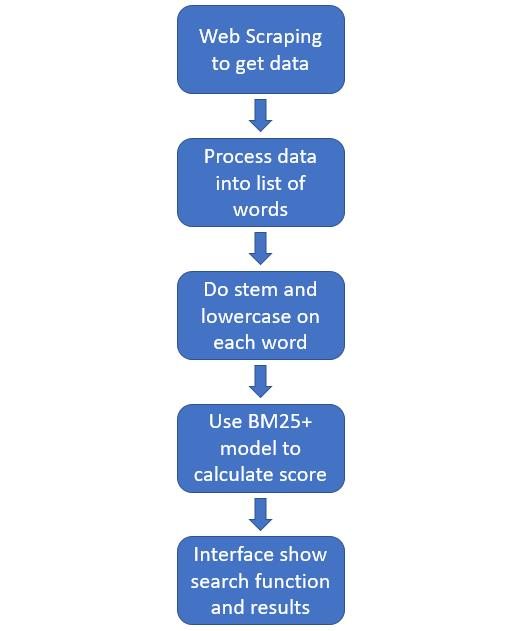
\includegraphics[width=0.5\linewidth]{process.jpg}
        \captionof{figure}{Working process of our searching system}
    \end{Figure}

    \subsection{Dataset}
    We obtained our data from two sources:

    Kaggle movie dataset:
    \url{(https://www.kaggle.com/rounakbanik/the-movies-dataset#movies_metadata.csv)}

    IMDB website
    \url{(https://www.imdb.com/?ref_=nv_home)}

    We first download a csv file from Kaggle with data about overviews and imdb link for each movie. We first try to use these overviews as documents for queries. Then we find that the performance of searching can't fulfill our satisfication so we try to find more documents. Finally, after tring the summary on wikipedia and total scene description on IMDB, we choose keywords on IMDB and use python webscraping to get these data.

    \subsection{Basic Data processing}

    In this project, our retrieval system is built to retrieve movie by its description and our data document for each movie contains its overview and keywords related to it.

    We first scrape keyword data from a website and combined it with the overview of each movie from the Kaggle dataset into one string. Then, we tokenize the string into words and do stem and lowercase on each word and get lists of words for each document. Finally we remove stopwords and punctuations, and  the document is then ready for query. The above mentioned steps are also applied to query sentences.

    \subsection{Advanced Data processing}

    We tried two advanced methods on data to see if the performance of search can be enhanced.

    First, we thought of adding the synonyms of each words in query so that those words with similar mean as query words in documents would not be missed. For each query we used nltk wordnet to get synonyms for each word in the query and added them into the query. However, the performance become worse instead of bettern. We thought that may be adding synouyms made the query vaguer so that more unrelated results are searched.

    Also, we thought of adding weight to different kind of words in query. But that will led to another question that how should we judge the importance of different words. We thought of using part-of-speech tagger to tag each words in query and give more weight to adjectives and verbs. However, there is no distince improvement in the performance of our system. We can do further improvement on our system by trying to find more proper weighting methods on queries.

    \subsection{Model}

    We first use BM25 score function which is use to give score to each query-document pair by the term frequency(TF) of each word in the query and inverse document frequency (IDF) as following:

    {
    \tiny
    $$
        S = \sum_{t \in q} \cdot\left[\frac{\left(k_{1}+1\right) \\ \cdot c_{t}^{d}}{c_{t}^{d}+k_{1} \cdot\left(1-b+b \cdot \frac{l_{d}}{L}\right)}\right] \cdot \ln \left(\frac{N+1}{N_{t}}\right)
    $$
    }

    However, the performance of BM25 score function is not so good so we want to find a more proper score function. We tried BM25+ function. The differences between BM25+ and BM25 are that BM25+ add an additional parameter and consider the frequency of each words in query. Since the performance of BM25+ is better and can relatively meet our needs, we finally choose it as our final score function (Inspiration from \url{https://www.eecis.udel.edu/~ypeilin/pub/ictir2016_long.pdf)} which is :

    {
    \tiny
    $$
        S = \sum_{t \in q} \frac{\left(k_{3}+1\right) \cdot c_{t}^{q}}{k_{3}+c_{t}^{q}} \cdot\left[\frac{\left(k_{1}+1\right) \\ \cdot c_{t}^{d}}{c_{t}^{d}+k_{1} \cdot\left(1-b+b \cdot \frac{l_{d}}{L}\right)}+\delta\right] \cdot \ln \left(\frac{N+1}{N_{t}}\right)
    $$
    }


    This BM25+ function add two more parameters to change the weight of TF and IDF in the function and it make our performance better in our test query set. The performance comparison and analysis will be detailedly discussed in Result and evaluation part.

    \subsection{Interface}

    We have also built an interface for users to input the description they remember and will return the result movie name and simple overview. The movie with best score will be shown on the page and user can see more results with lower scores if he slide down the page as following graphs:

    \begin{Figure}
        \center
        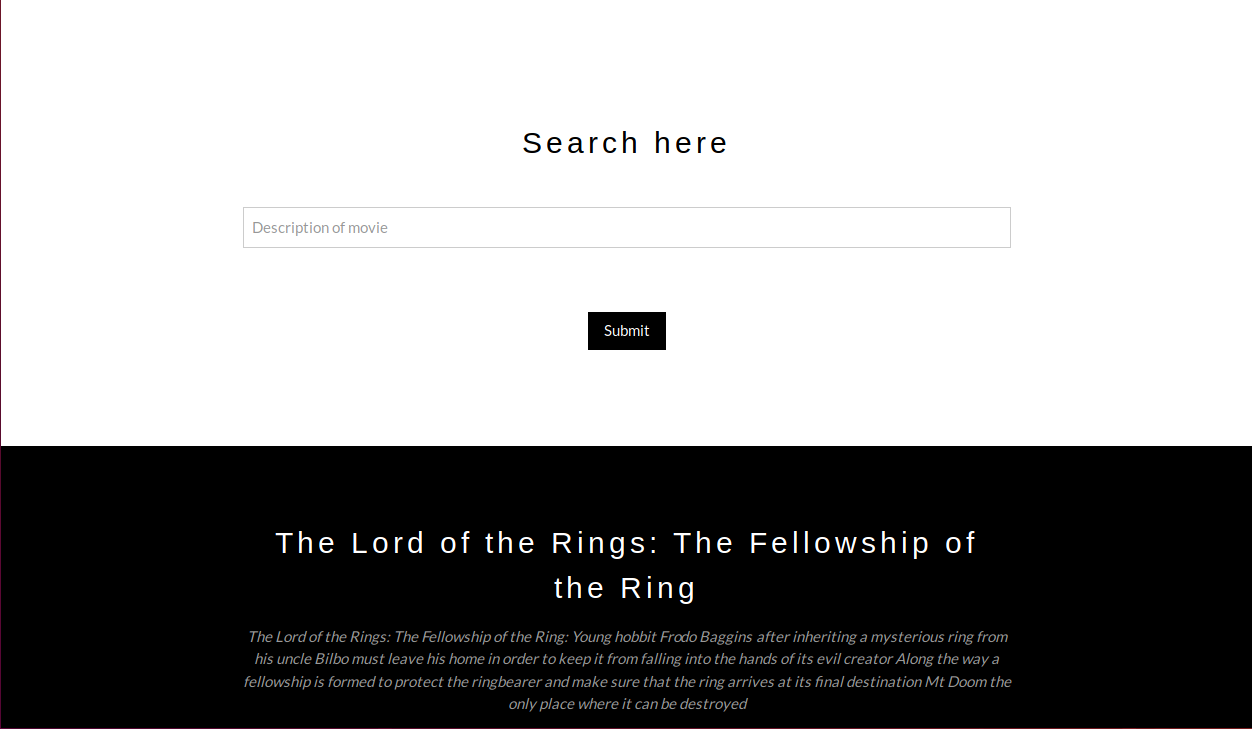
\includegraphics[width=0.8\linewidth]{interface.jpg}
        \captionof{figure}{Interface}
    \end{Figure}

    \begin{Figure}
        \center
        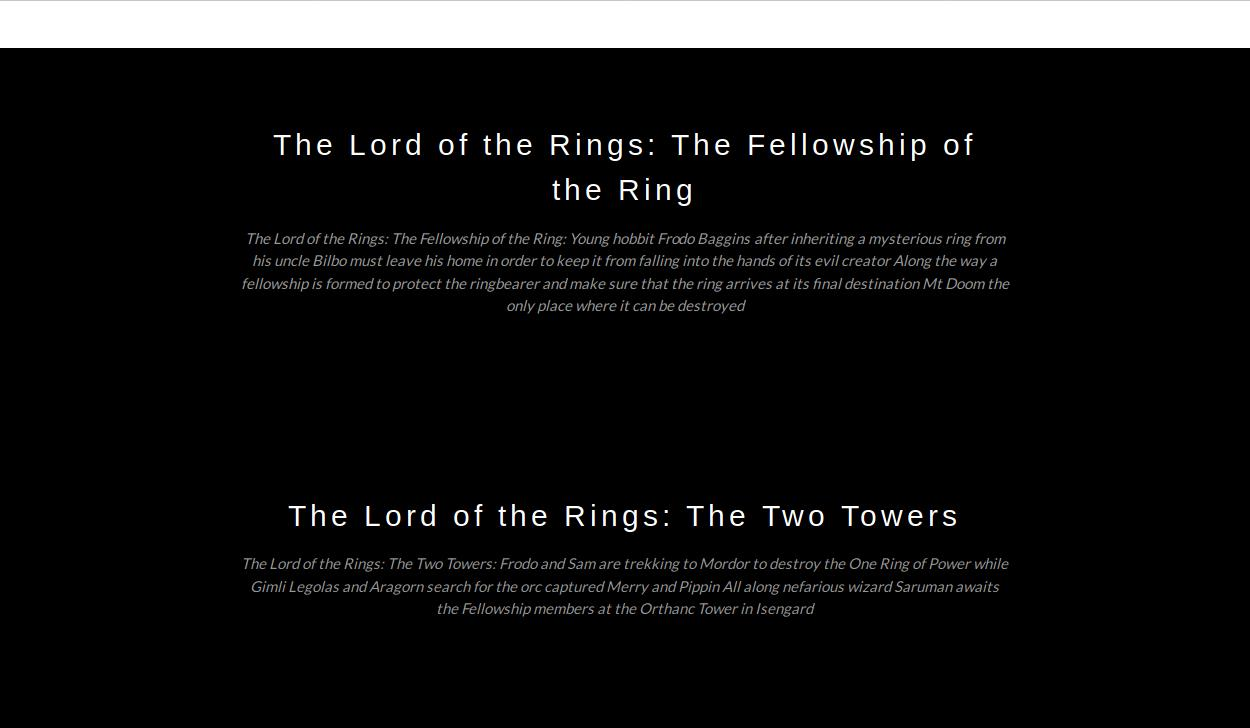
\includegraphics[width=0.8\linewidth]{interface1.jpg}
        \captionof{figure}{Interface slide down}
    \end{Figure}

    \section{Results and evaluation}

    We formulate 35 short descriptions of movies and use our search engine to
    fetch the result.
    Some of the queries come from us and some of them are from our user during
    the testing phase of our development.
    For each description, we check if the intended result is returned by the
    search engine.

    Then we check the rank $R$ of the expected movie returned by the search
    engine.
    We define $\frac{1}{R}$ as the precision of our search engine.
    We calculate the harmonic mean of $R$ (if the expected movie isn’t retrieved
    within the first 10 movies, R is infinity.) and use it as the evaluation for
    the search engine.

    This is part of the testing result from our search engine, the third coloum
    is the rank of the movie title retrieved based on BM25 BM25 and the fourth
    coloum is for BM25+.

    \begin{Figure}
        \centering
        \begin{tabular}{ |l | l |l|l|} \hline
            Query             & Answer         & $\frac{R}{\text{BM25}}$ & $\frac{R}{\text{BM25+}}$ \\ \hline
            Jack and rose     & Titanic        & 2                       & 1                        \\ \hline
            Dinosaur          & Jurassic World & 4                       & 1                        \\ \hline
            France revolution & Les Misérables & 4                       & 2                        \\ \hline
            Dream thief       & Inception      & 6                       & 1                        \\ \hline
            Boy magic school  & Harry Potter   & 9                       & 1                        \\ \hline
            Cowboy astronaut  & Toy story      & 5                       & 1                        \\ \hline
            Robot kill human  & Terminator     & 4                       & 1                        \\ \hline
        \end{tabular}
        \captionof{figure}{Part of Our Queries Test Result}
    \end{Figure}


    The harmonic mean of rank of the expected movies can evaluate the average
    results the user need to skim through to find the movie they intend to have.
    Thus, the lower harmonic mean of rank, the better engine we have.
    The following is the harmonic mean of rank result of BM25 and BM25+.

    \begin{Figure}
        \centering
        \begin{tabular}{ |c | c |c|}
            \hline
                                                           & BM25  & BM25+ \\ \hline
            $\frac{n}{\sum_{i=1}^{i=n} \frac{1}{R_{i}} } $ & 2.944 & 1.449 \\  \hline
        \end{tabular}
        \captionof{figure}{Comparison of Harmonic Mean of Rank }
    \end{Figure}

    The following is the figure showing the sorted distribution of expected movie retrieved ranks.
    For the figure for BM25, there are a lot of queries that returns failure (greater than 10),
    while for BM25+, there is no failure and the mean of ranks is obviously lower.

    \begin{Figure}
        \center
        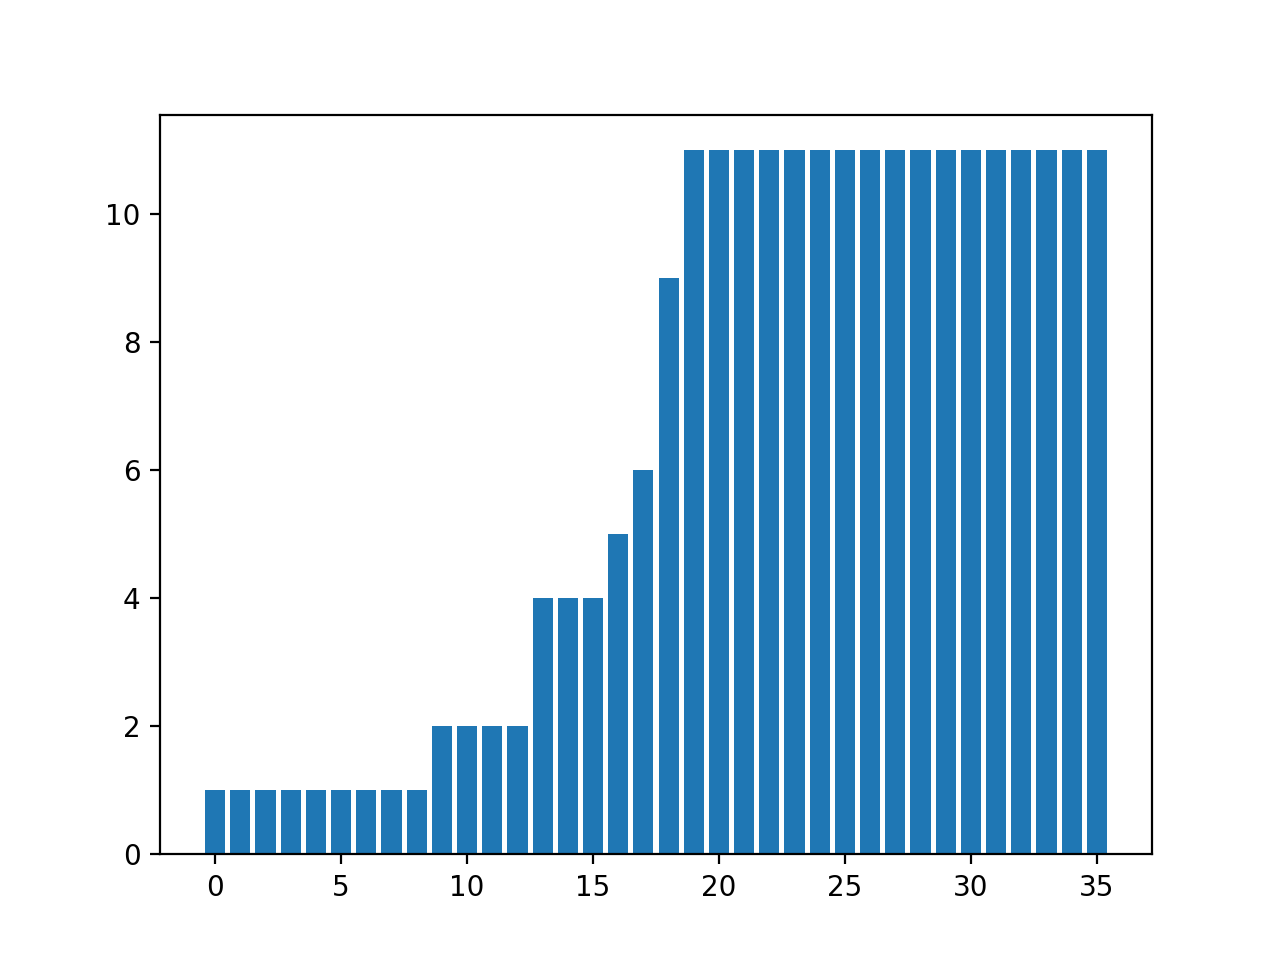
\includegraphics[width=0.47\linewidth]{evaluation_1.png}
        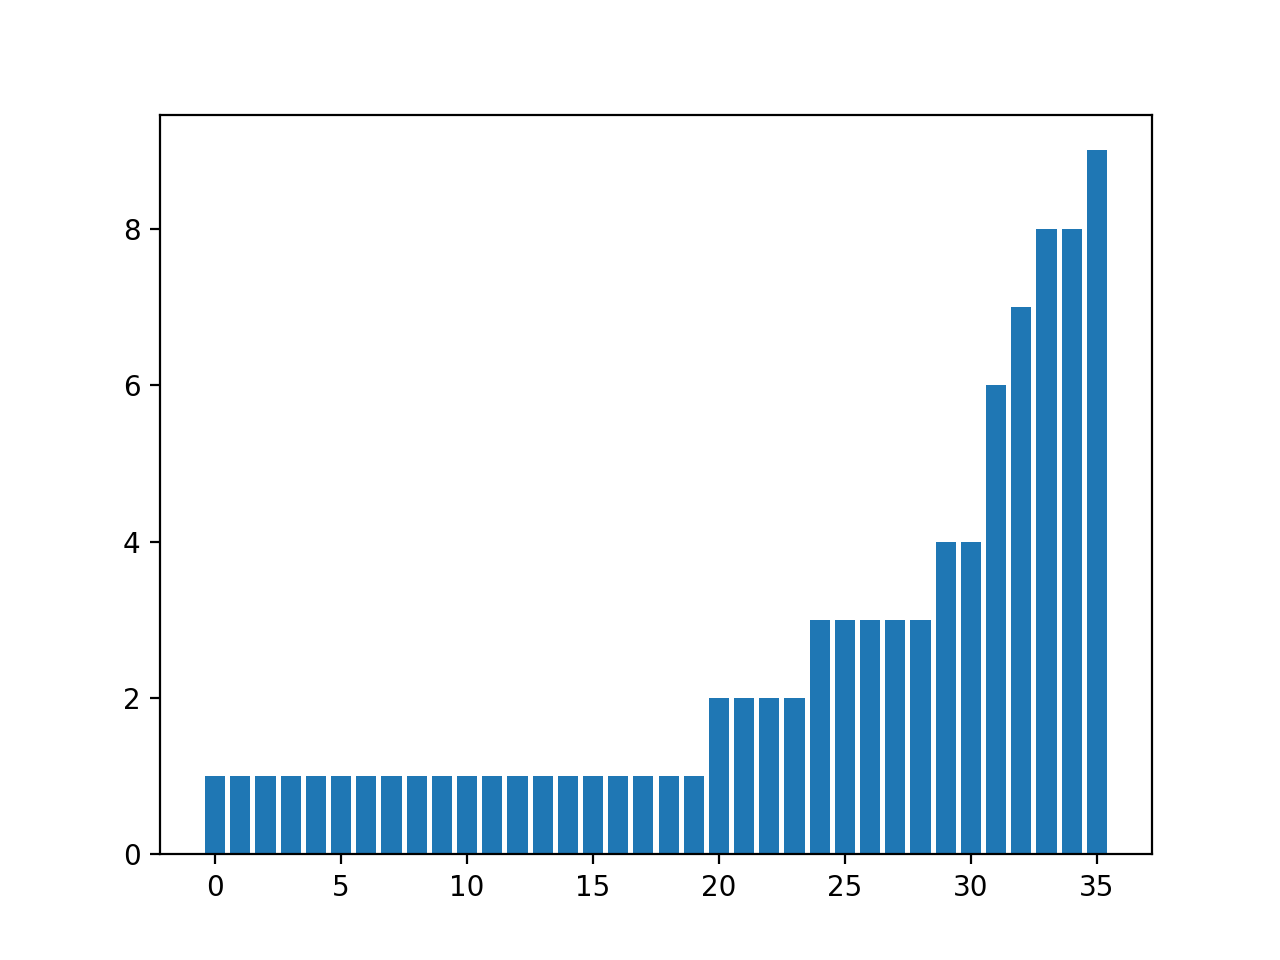
\includegraphics[width=0.47\linewidth]{evaluation_2.png}
        \captionof{figure}{Expected Movie Retreived Ranks Distribution}
    \end{Figure}

    Thus we can evaluate our search engine as useful, for on average the user
    can expect to find the moive they want from the first and second result
    retrieved.

    \subsection{Comparison between our search engine and Google}

    It's hard to quantatively compare our search engine's capability with
    Google, because for each query, Google returns results of webpages, images
    and even links to external websites.
    However, the common behavior of Google is to treat the query ``as it is''. 
    For example, when the user wants to find the movie ``Jurassic World'' when he or she only remembers
    scenes of Dinosaurs, Google will return some sophisticated documentary
    movies of ``Dinosaur'', but what the user really want is ``a popular movie in
    which dinosaurs show up''. 
    Thus, for accomplishing the job of searching movie based on fragments of description, our search engine
    can beat Google.

    \section{Conclusions}

    The result of this project is generally satisfying with our experiments with
    it. We succeeded in returning the related results with the queries and has
    improved its performance with data processing and parameter tuning. Thus,
    with our search engine, people can mostly get the movie they referred to.
    However, the search engine might not work well with subjective feelings on
    movies since the data we used for query are neutral descriptions.

    \section{Future Improvements}
    During data processing, we have tried part of speech tagging on the sentence and give more weights to certain types. However, it doesn’t turn out well as we expected. We believe that digging further into this by analyzing the parse tree to evaluate the part of speeches more precisely can help with giving better weights.
    Moreover, we believe that keeping a search and view log can also help with improving accuracy. Within a series of similar searches, we can analyze the movies the user has clicked into and find the similarities to feed back into the algorithm and adjust the weights accordingly.

    \section{Acknowledgement}

    Prof. Qiaozhu Mei, Mr. Wei Ai from University of Michigan;
    Teaching Assistant [Shiyan Yan, Xinyan Zhao] for SI 650 at University of Michigan.

    \section*{References}





\end{multicols}

\end{document}
